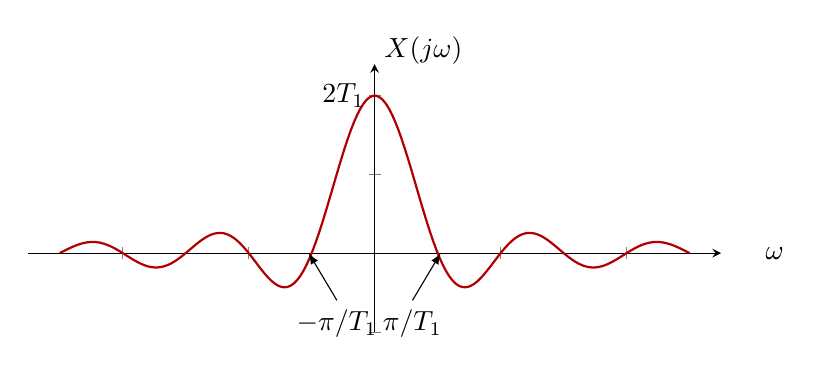
\begin{tikzpicture}
    \begin{axis}[
		y=2cm,
		x=0.8cm,
		 clip=false,
		 xmin=-5.5,xmax=5.5,
		 xlabel= $\omega$,
		 ylabel={$X(j\omega)$},
		 ymin=-0.5,ymax=1.2,
		 axis lines=middle,
         	%xtick={-5, -4, ..., 5},
		 %ytick={-1, 1},
		 yticklabels=\empty,
		 xticklabels=\empty,
		 every axis x label/.style={at={(ticklabel* cs:1.05)}, anchor=west,},
		every axis y label/.style={at={(ticklabel* cs:1.05)}, anchor=west,},
     ]
		%\addplot+[red, smooth, mark=none] table [x={n}, y={xn}] {periodic_square_fs_samples_of_envilope_gen.dat};
		\addplot [red!70!black, thick, domain=-5:5, samples=200] plot{sin(pi*deg(x))/(pi*x)};
		\node at (axis cs:0, 1) [anchor=east] { $2T_1$ };
		\draw[latex-] (axis cs:pi/3, 0) --(axis cs:0.6,-0.3) node  [anchor=north] { $\pi/T_1$ } ;
		\draw[latex-] (axis cs:-pi/3, 0) --(axis cs:-0.6,-0.3) node  [anchor=north] { $-\pi/T_1$ } ;		
    \end{axis}
\end{tikzpicture} 